\section{Spark Streaming}\label{s:spark-streaming}

\FILENAME\

\subsection{Streaming Concepts}

Spark Streaming is one of the components extending from Core Spark.
Spark streaming provides a scalable fault tolerant system with high
throughput. For streaming data into spark, there are many libraries
like Kafka, Flume, Kinesis, etc.

\subsection{Simple Streaming Example}

In this section, we are going to focus on making a simple streaming
application using the network in your computer. Here we are going to
expose a particular port and from that port we are going to
continously stream data by user entries and the word count is being
calculated as the output.

First, create a Makefile

\begin{lstlisting}
  mkdir -p ~/cloudmesh/spark/examples/streaming
  cd ~/cloudmesh/spark/examples/streaming
  emacs Makefile
\end{lstlisting}

Then add the following content to Makefile. 
\begin{NOTE}
  Please add a tab when adding the corresponding command for a given instruction
  in Makefile. In pdf mode the tab is not clearly shown. 
\end{NOTE}
\begin{lstlisting}
  SPARKHOME = ${SPARK_HOME}
  run-streaming:
	${SPARKHOME}/bin/spark-submit streaming.py localhost 9999
\end{lstlisting}
      
Now we need to create file called streaming.py

\begin{lstlisting}
  emacs streaming.py
\end{lstlisting}

Then add the following content. 

\begin{lstlisting}
from pyspark import SparkContext
from pyspark.streaming import StreamingContext

# Create a local StreamingContext with two working thread and batch interval of 1 second
sc = SparkContext("local[2]", "NetworkWordCount")

log4jLogger = sc._jvm.org.apache.log4j
LOGGER = log4jLogger.LogManager.getLogger(__name__)
LOGGER.info("Pyspark script logger initialized")

ssc = StreamingContext(sc, 1)


# Create a DStream that will connect to hostname:port, like localhost:9999
lines = ssc.socketTextStream("localhost", 9999)
# Split each line into words
words = lines.flatMap(lambda line: line.split(" "))
# Count each word in each batch
pairs = words.map(lambda word: (word, 1))
wordCounts = pairs.reduceByKey(lambda x, y: x + y)

# Print the first ten elements of each RDD generated in this DStream to the console
wordCounts.pprint()
ssc.start()             # Start the computation
ssc.awaitTermination(100)  # Wait for the computation to terminate

\end{lstlisting}

To run the code, we need to open up two terminals.

\verb|Terminal 1 :|

First use netstat to open up a port to start communication.

\begin{lstlisting}
  nc -lk 9999
\end{lstlisting}


\verb|Terminal 2 :|

Now run the Spark programme in the second terminal.

\begin{lstlisting}
  make run-streaming
\end{lstlisting}

In this terminal you can see an script running trying to read
the stream coming from the port 9999. You can enter texts in the
Terminal 1 and these texts will be tokenized and the word count is
calculated and the result is shown in the Terminal 2.

\subsection{Spark Streaming For Twitter Data}

In this section we are going to learn how to use Twitter data as the streaming data source and use Spark Streaming capabilities to process the data. As the first step you must install the python packages using pip.

\subsubsection{Step 1}

\begin{lstlisting}
  sudo pip install tweepy
\end{lstlisting}

\subsubsection{Step 2}

Then you need to create an account in Twitter Apps. Go to
\URL{https://apps.twitter.com/} and sign in to your twitter account or
create a new twitter account. Then you need to create a new application,
let's name this application as \verb|Cloudmesh-Spark-Streaming|.

First you need to create an app with the app name we suggested in this
section. The way to create the app is mentioned in Figure \ref{fig:twitter-app}.

\begin{figure}[htbp]\label{fig:twitter-app}
\centering
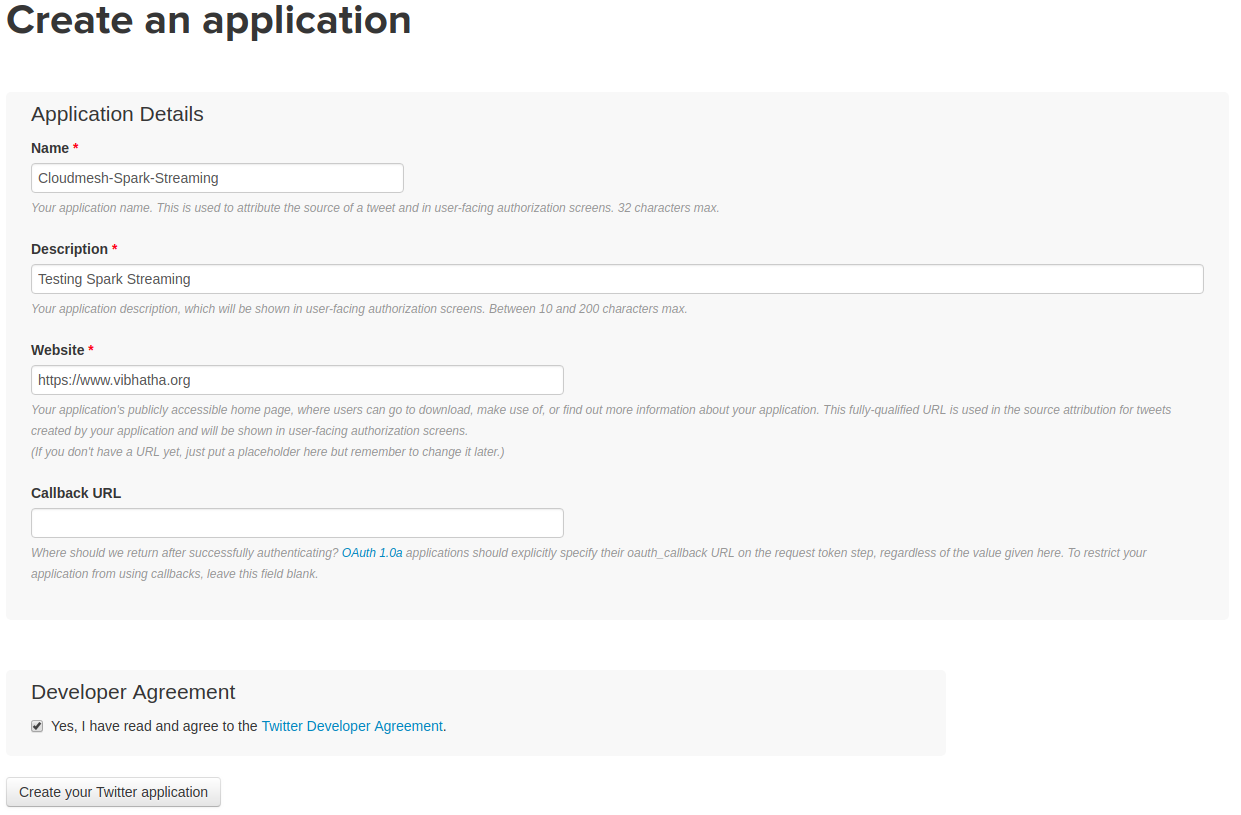
\includegraphics[width=1.0\textwidth]{images/twitter-app.png}
\caption{Create Twitter App}
\end{figure}

Next we need to to take a look at the dashboard created for the app.
You can see how your dashboard looks like in Figure \ref{fig:twitter-app-dashboard}. 

\begin{figure}[htbp]\label{fig:twitter-app-dashboard}
\centering
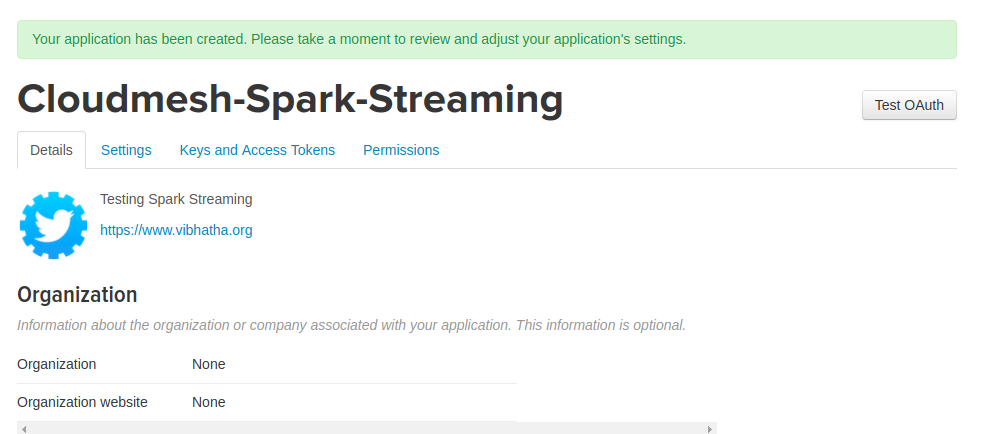
\includegraphics[width=1.0\textwidth]{images/twitter-app-dashboard.png}
\caption{Go To Twitter App Dashboard}
\end{figure}

Next the application tokens generated must be reviewed and it can be
found in Figure \ref{fig:twitter-app-token}, you need to go to the
\verb|Keys and Access Tokens| tab.

\begin{figure}[htbp]\label{fig:twitter-app-token}
\centering
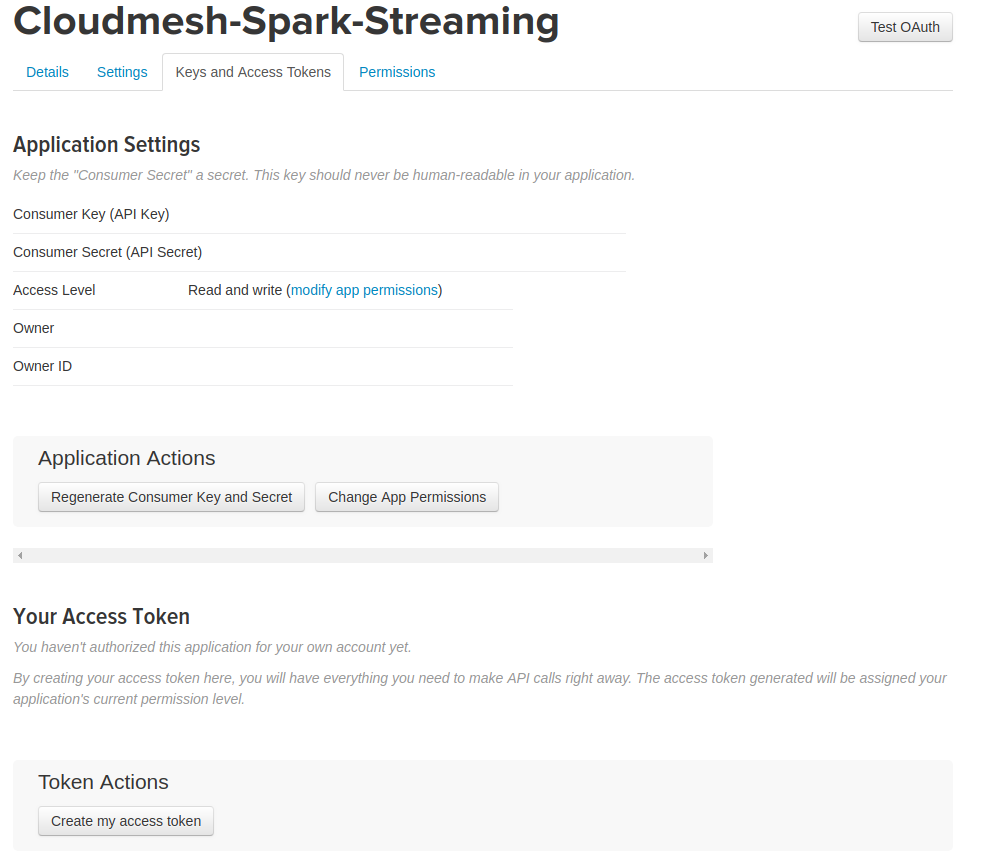
\includegraphics[width=1.0\textwidth]{images/twitter-create-token.png}
\caption{Create Your Twitter Settings}
\end{figure}

Now you need to generate the access tokens for the first time if you
have not generated access tokens and this can be done by clicking the
\verb|Create my access token| button.

\begin{figure}[htbp]\label{fig:twitter-app-access-token}
\centering
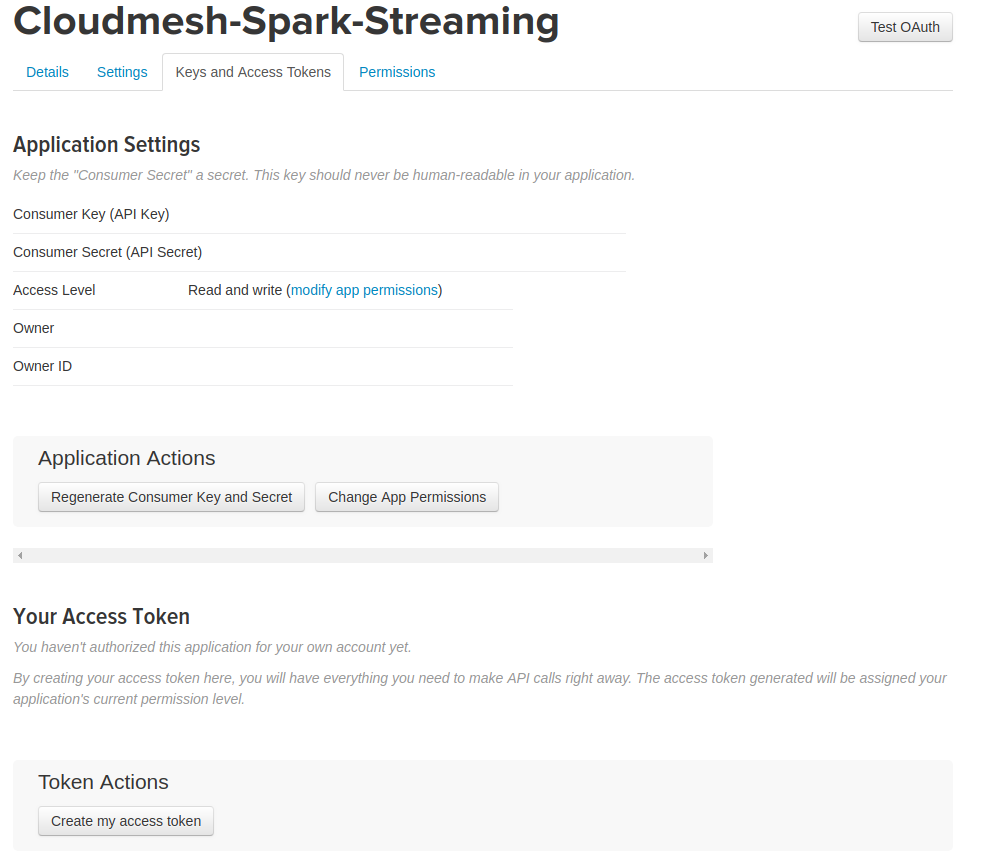
\includegraphics[width=1.0\textwidth]{images/twitter-create-token.png}
\caption{Create Your Twitter Access Tokens}
\end{figure}

\begin{NOTE}
The access tokens and keys are blurred in this section for privacy issues.   
\end{NOTE}

\subsubsection{Step 3}

Let us build a simple Twitter App to see if everything is okay.

\begin{lstlisting}
  mkdir -p ~/cloudmesh/spark/streaming
  cd ~/cloudmesh/spark/streaming
  emacs twitterstreaming.py
\end{lstlisting}

Add the following content to the file and make sure you update the
corresponding token keys with your token values.

\begin{lstlisting}
import tweepy

CONSUMER_KEY = 'your_consumer_key'
CONSUMER_SECRET = 'your_consumer_secret'
ACCESS_TOKEN = 'your_access_token'
ACCESS_TOKEN_SECRET = 'your_access_token_secret'

auth = tweepy.OAuthHandler(CONSUMER_KEY, CONSUMER_SECRET)
auth.set_access_token(ACCESS_TOKEN, ACCESS_TOKEN_SECRET)
api = tweepy.API(auth)

status = "Testing!"
api.update_status(status=status)
\end{lstlisting}

\begin{lstlisting}
  python twitterstreaming.py
\end{lstlisting}

\subsubsection{Step 4}

Let us start the twitter streaming exercise. We need to create a Tweet
Listener in order to retrieve data from twitter regarding a topic of
your choice. In this exercise, we have tried keywords like
\verb|trump, indiana, messi|.

\begin{lstlisting}
  mkdir -p ~/cloudmesh/spark/streaming
  cd ~/cloudmesh/spark/streaming
  emacs tweetlistener.py
\end{lstlisting}

\begin{NOTE}
  Make your to replace strings related to secret keys and ip addresses
  by replacing these values depending on your machine configuration
  and twitter keys.
\end{NOTE}

Now add the following content.

\begin{lstlisting}
import tweepy
from tweepy import OAuthHandler
from tweepy import Stream
from tweepy.streaming import StreamListener
import socket
import json

CONSUMER_KEY = 'YOUR_CONSUMER_KEY'
CONSUMER_SECRET = 'YOUR_CONSUMER_SECRET'
ACCESS_TOKEN = 'YOUR_ACCESS_TOKEN'
ACCESS_SECRET = 'YOUR_SECRET_ACCESS'

class TweetListener(StreamListener):

  def __init__(self, csocket):      
      self.client_socket = csocket

  def on_data(self, data):
      try:
          msg = json.loads( data )
          print( msg['text'].encode('utf-8') )
          self.client_socket.send( msg['text'].encode('utf-8') )
          return True
      except BaseException as e:
          print("Error on_data: %s" % str(e))
      return True

  def on_error(self, status):
      print(status)
      return True

def sendData(c_socket):
  auth = OAuthHandler(CONSUMER_KEY, CONSUMER_SECRET)
  auth.set_access_token(ACCESS_TOKEN, ACCESS_SECRET)

  twitter_stream = Stream(auth, TweetListener(c_socket))
  twitter_stream.filter(track=['messi']) # you can change this topic 

if __name__ == "__main__":
  s = socket.socket()         
  host = "YOUR_MACHINE_IP"      
  port = 5555              
  s.bind((host, port))     

  print("Listening on port: %s" % str(port))

  s.listen(5)              
  c, addr = s.accept()     

  print( "Received request from: " + str( addr ) )

  sendData( c )

\end{lstlisting}


\subsubsection{step 5}

\begin{NOTE}
  Please replace the local file paths mentioned in this code with a
  file path of your preference depending on your workstation. And also
  IP address must be replaced with your ip address. The log folder
  path must be pre-created and makesure to replace the
  \verb|registerTempTable| name with respect to the entity that you
  are referring. This will minimize the conflicts among different
  topics when you need to plot it in a simple manner.
\end{NOTE}

Add the following content to the IpythonNote book as follows

Open up a terminal,

\begin{lstlisting}
  cd ~/cloudmesh/spark/streaming
  jupyter notebook
\end{lstlisting}

Then in the browser the jupyter notebook is being loaded.  There
create a new Ipython notebook called twittersparkstremer.

Then add the following content. 

\begin{lstlisting}
from pyspark import SparkContext
from pyspark.streaming import StreamingContext
from pyspark.sql import SQLContext
from pyspark.sql.functions import desc
\end{lstlisting}

\begin{lstlisting}
sc = SparkContext('local[2]','twittersparkstreamer')
\end{lstlisting}

\begin{lstlisting}
ssc = StreamingContext(sc, 10 )
sqlContext = SQLContext(sc)
ssc.checkpoint( "file:///home/<your-username>/cloudmesh/spark/streaming/logs/messi")
\end{lstlisting}

\begin{lstlisting}
socket_stream = ssc.socketTextStream("YOUR_IP_ADDRESS", 5555)
\end{lstlisting}

\begin{lstlisting}
lines = socket_stream.window( 20 )
\end{lstlisting}

\begin{lstlisting}
from collections import namedtuple
fields = ("tag", "count" )
Tweet = namedtuple( 'Tweet', fields )
\end{lstlisting}

\begin{lstlisting}
( lines.flatMap( lambda text: text.split( " " ) )
  .filter( lambda word: word.lower().startswith("#") )
  .map( lambda word: ( word.lower(), 1 ) )
  .reduceByKey( lambda a, b: a + b )
  .map( lambda rec: Tweet( rec[0], rec[1] ) )
  .foreachRDD( lambda rdd: rdd.toDF().sort( desc("count") )
              .limit(10).registerTempTable("tweetsmessi") ) )#change table name depending on your entity
\end{lstlisting}

\begin{lstlisting}
sqlContext
\end{lstlisting}

\begin{lstlisting}
<pyspark.sql.context.SQLContext at 0x7f51922ba350>
\end{lstlisting}

\begin{lstlisting}
ssc.start()  
\end{lstlisting}

\begin{lstlisting}
import matplotlib.pyplot as plt
import seaborn as sn
\end{lstlisting}

\begin{lstlisting}
import time
from IPython import display


count = 0
while count < 10:
  time.sleep( 20 )
  top_10_tweets = sqlContext.sql( 'Select tag, count from tweetsmessi' ) #change table name according to your entity 
  top_10_df = top_10_tweets.toPandas()
  display.clear_output(wait=True)  
  #sn.figure( figsize = ( 10, 8 ) )
  sn.barplot( x="count", y="tag", data=top_10_df)
  plt.show()
  count = count + 1
\end{lstlisting}

\begin{lstlisting}
ssc.stop()
\end{lstlisting}

\subsubsection{step 6}

Open \verb|Terminal 1|, then do the following

\begin{lstlisting}
  cd ~/cloudmesh/spark/streaming
  python tweetslistener.py 
\end{lstlisting}

It will show that:

\begin{lstlisting}
     Listening on port: 5555
\end{lstlisting}


Open \verb|Terminal 2|

Now we must start the Spark app by running the content in the IPython Notebook by pressing \verb|SHIFT-ENTER| in each box to run each command.
Make sure not to run twice the starting command of the SparkContext or initialization of SparkContext.

Now you will see streams in the \verb|Terminal 1| and you can see plots after a while in the IPython Notebook.

Sample outputs can be seen in the Figures \ref{fig:twitter-out-1}, \ref{fig:twitter-out-2}, \ref{fig:twitter-out-3}, \ref{fig:twitter-out-4}.

\begin{figure}[htbp]\label{fig:twitter-out-1}
\centering
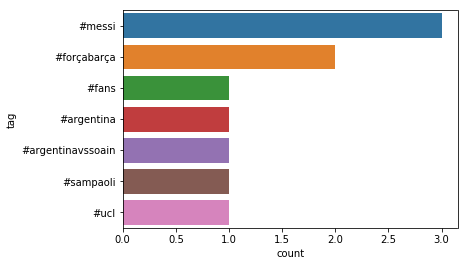
\includegraphics[width=1.0\textwidth]{images/twitter-messi-3.png}
\caption{Twitter Topic Messi}
\end{figure}


\begin{figure}[htbp]\label{fig:twitter-out-2}
\centering
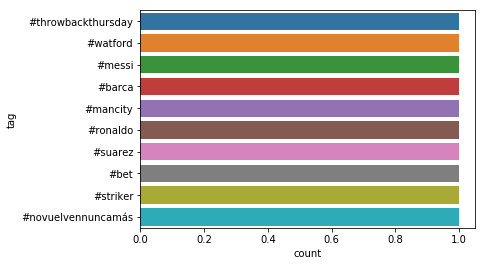
\includegraphics[width=1.0\textwidth]{images/twitter-messi-5.png}
\caption{Twitter Topic Messi}
\end{figure}

\begin{figure}[htbp]\label{fig:twitter-out-3}
\centering
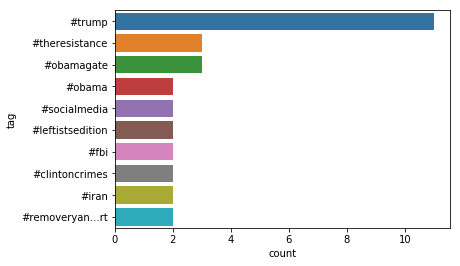
\includegraphics[width=1.0\textwidth]{images/twitter-trump-output.png}
\caption{Twitter Topic Messi}
\end{figure}


\begin{figure}[htbp]\label{fig:twitter-out-4}
\centering
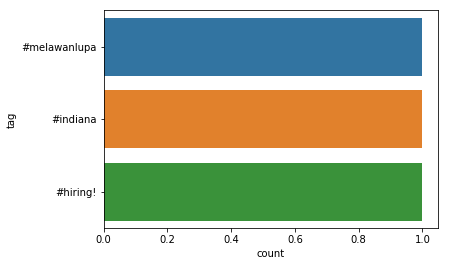
\includegraphics[width=1.0\textwidth]{images/twitter-indiana-2.png}
\caption{Twitter Topic Messi}
\end{figure}
